\appendix % Rozpoczęcie dodatków

\chapter{Dodatek: Schemat elektryczny}
\begin{figure}[H]
    \centering
    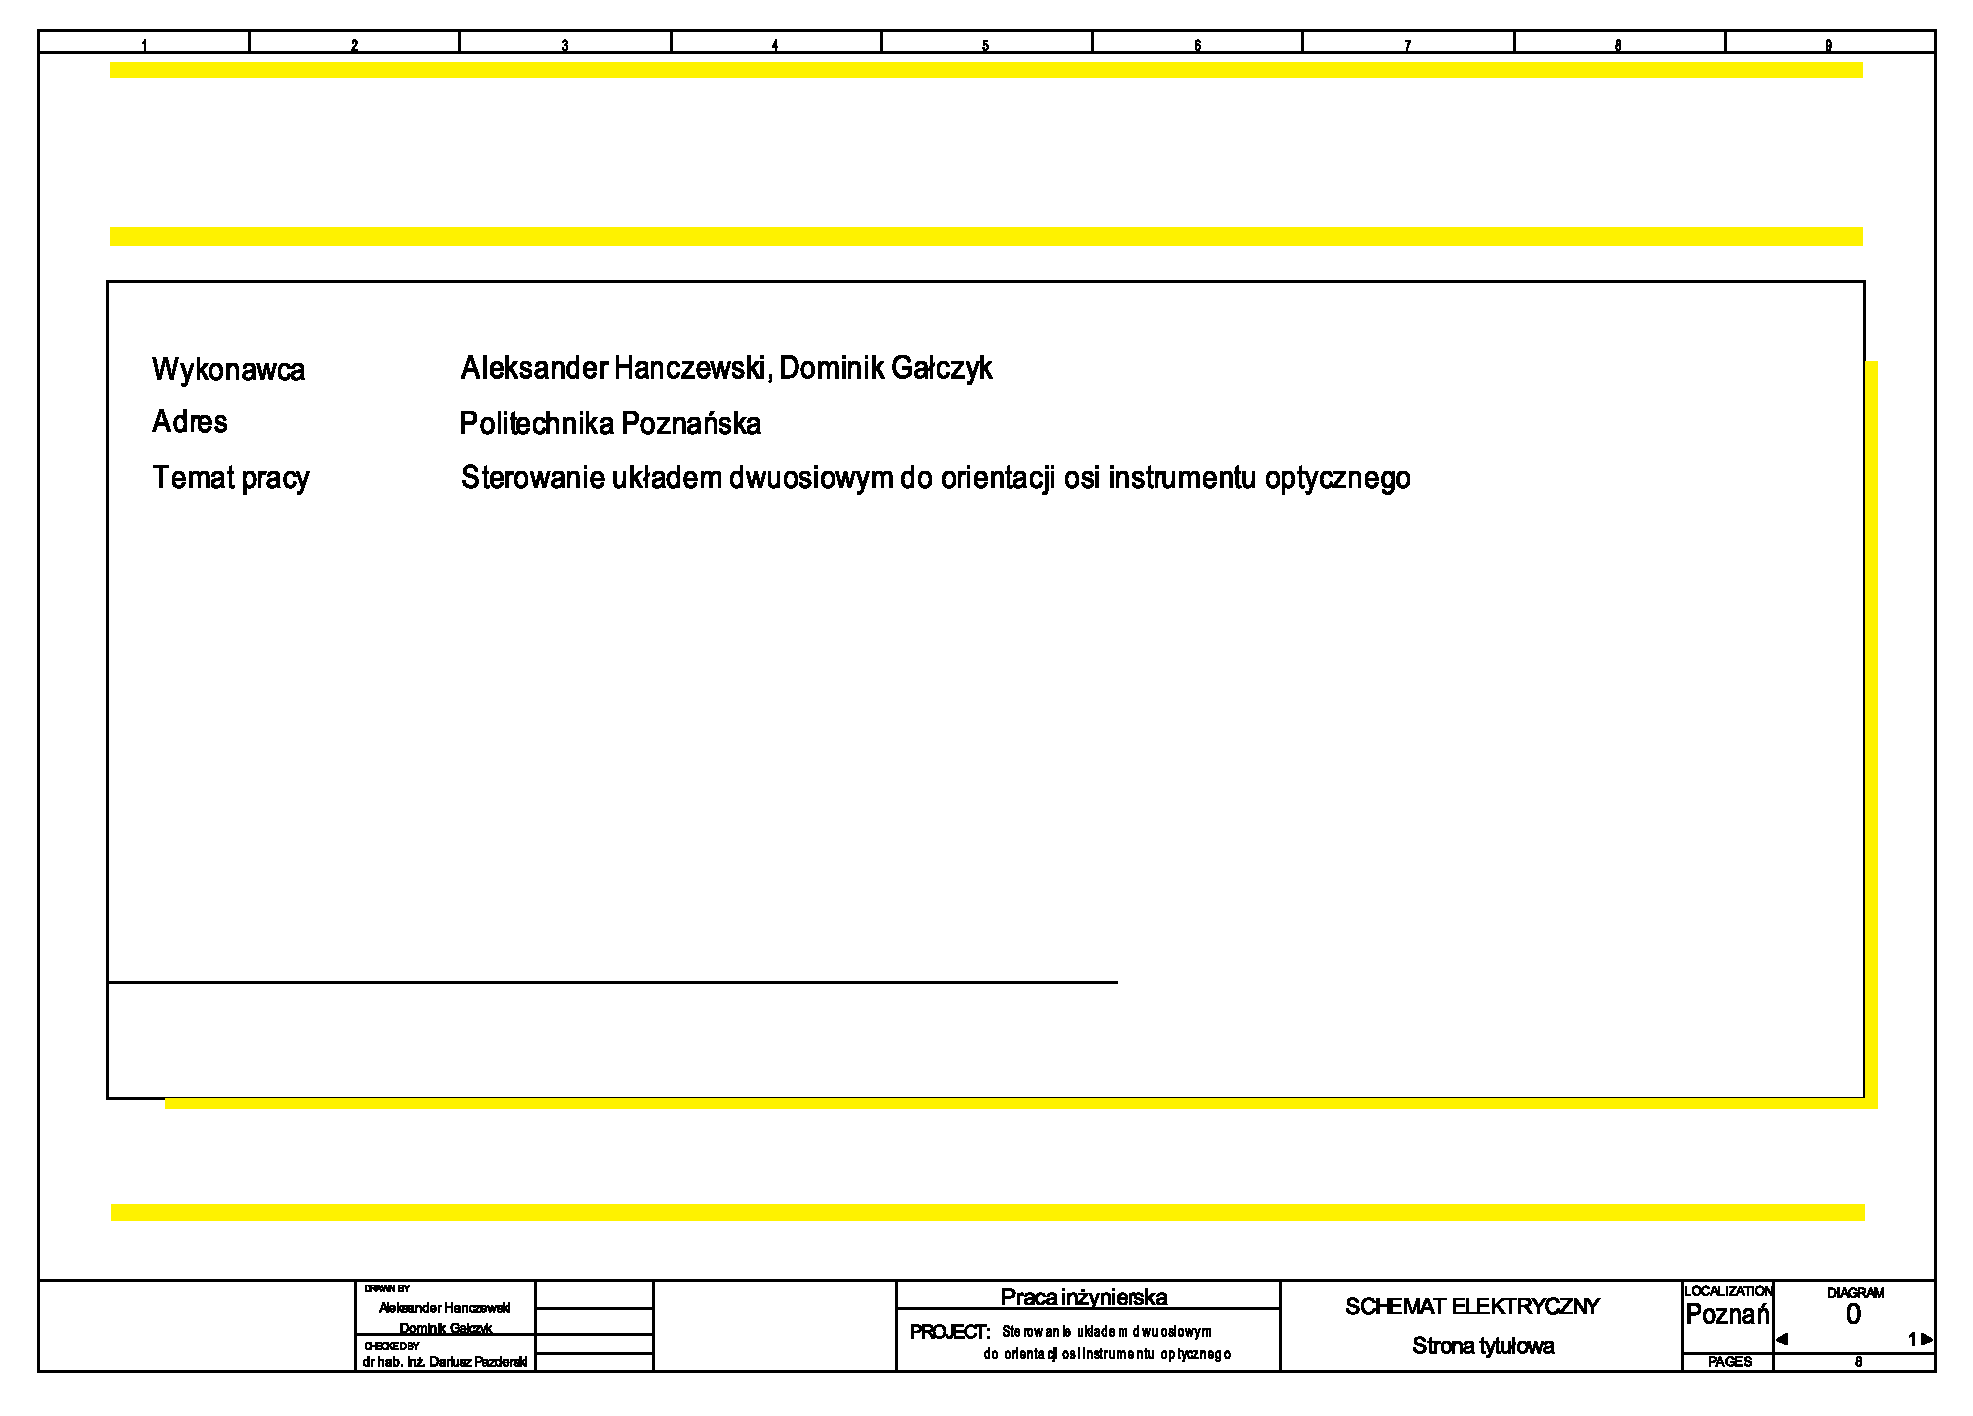
\includegraphics[width=0.85\textwidth]{pictures/schemat_elektryczny/Inżynierka (5).pdf}
\end{figure}

\begin{figure}[H]
    \centering
    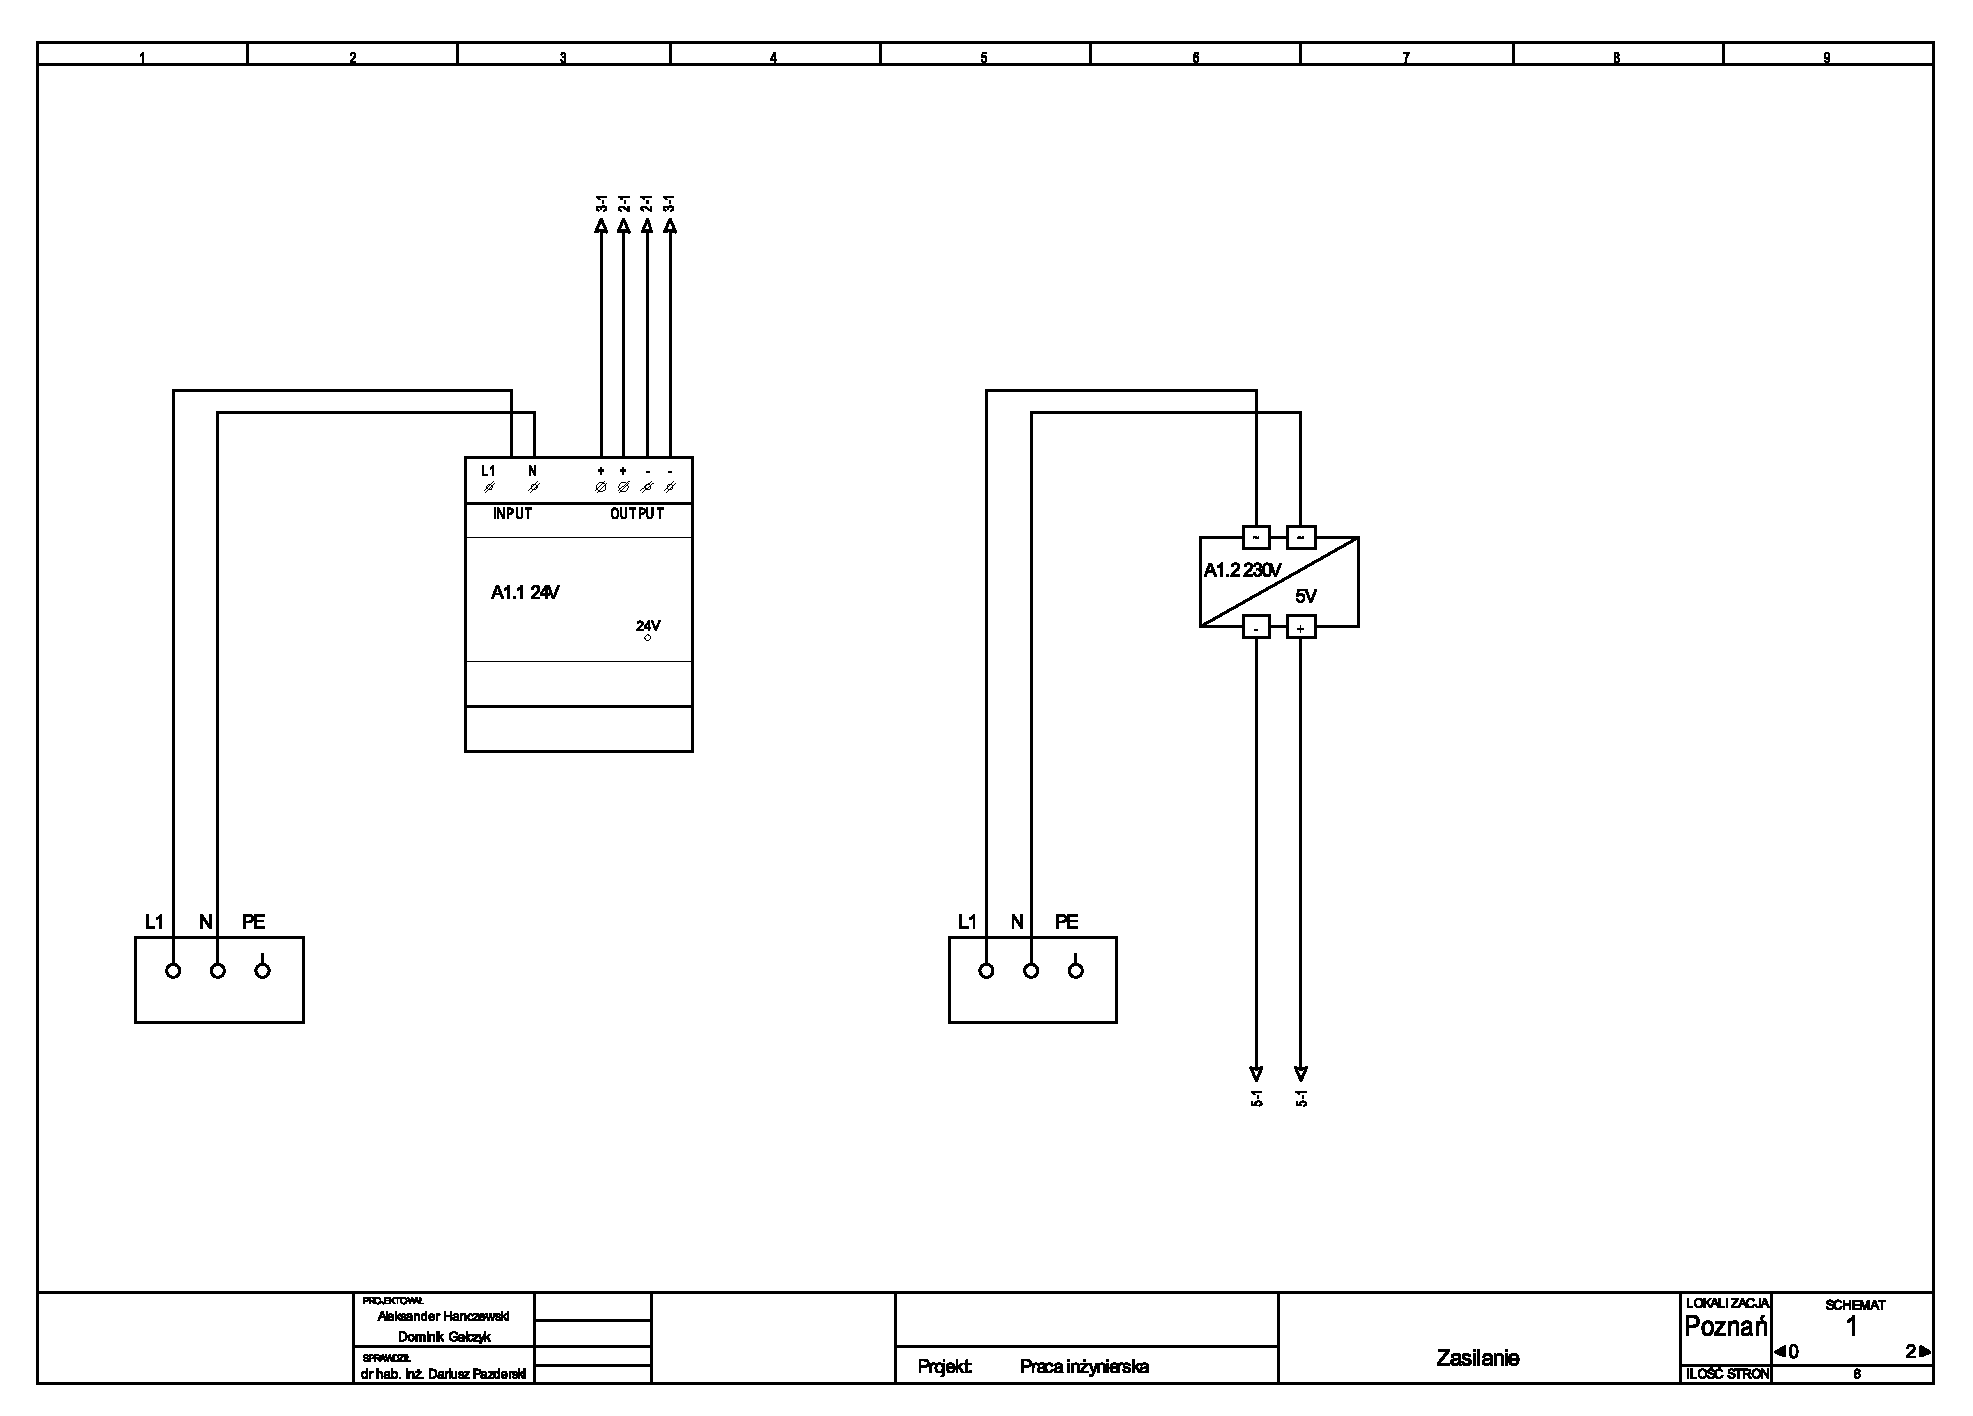
\includegraphics[width=0.85\textwidth]{pictures/schemat_elektryczny/Inżynierka (6).pdf}
\end{figure}

\begin{figure}[H]
    \centering
    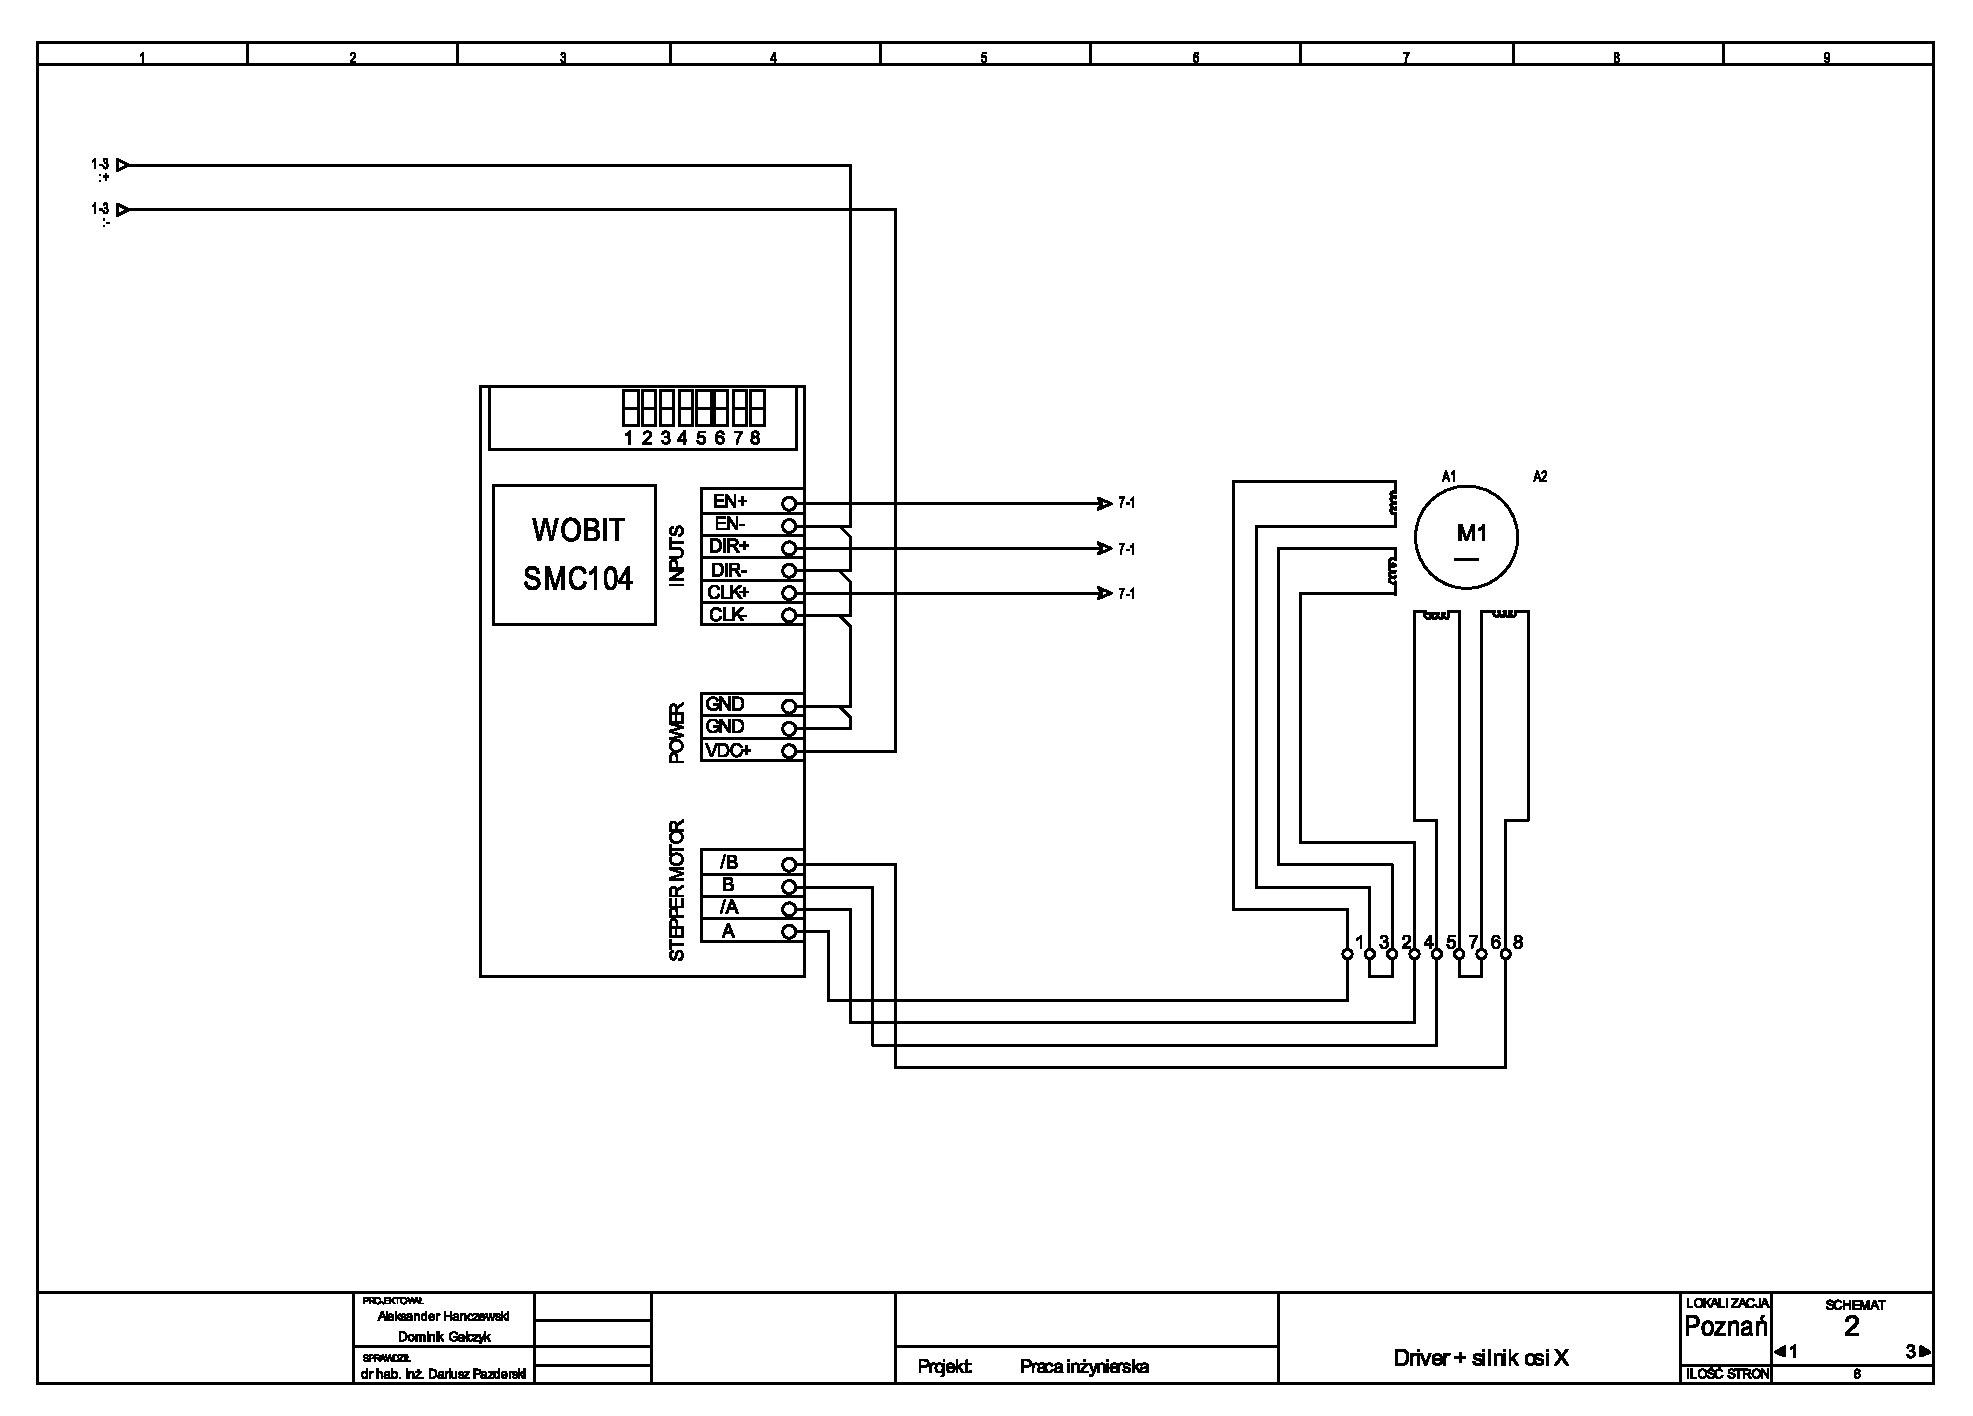
\includegraphics[width=0.85\textwidth]{pictures/schemat_elektryczny/Inżynierka (7).pdf}
\end{figure}

\begin{figure}[H]
    \centering
    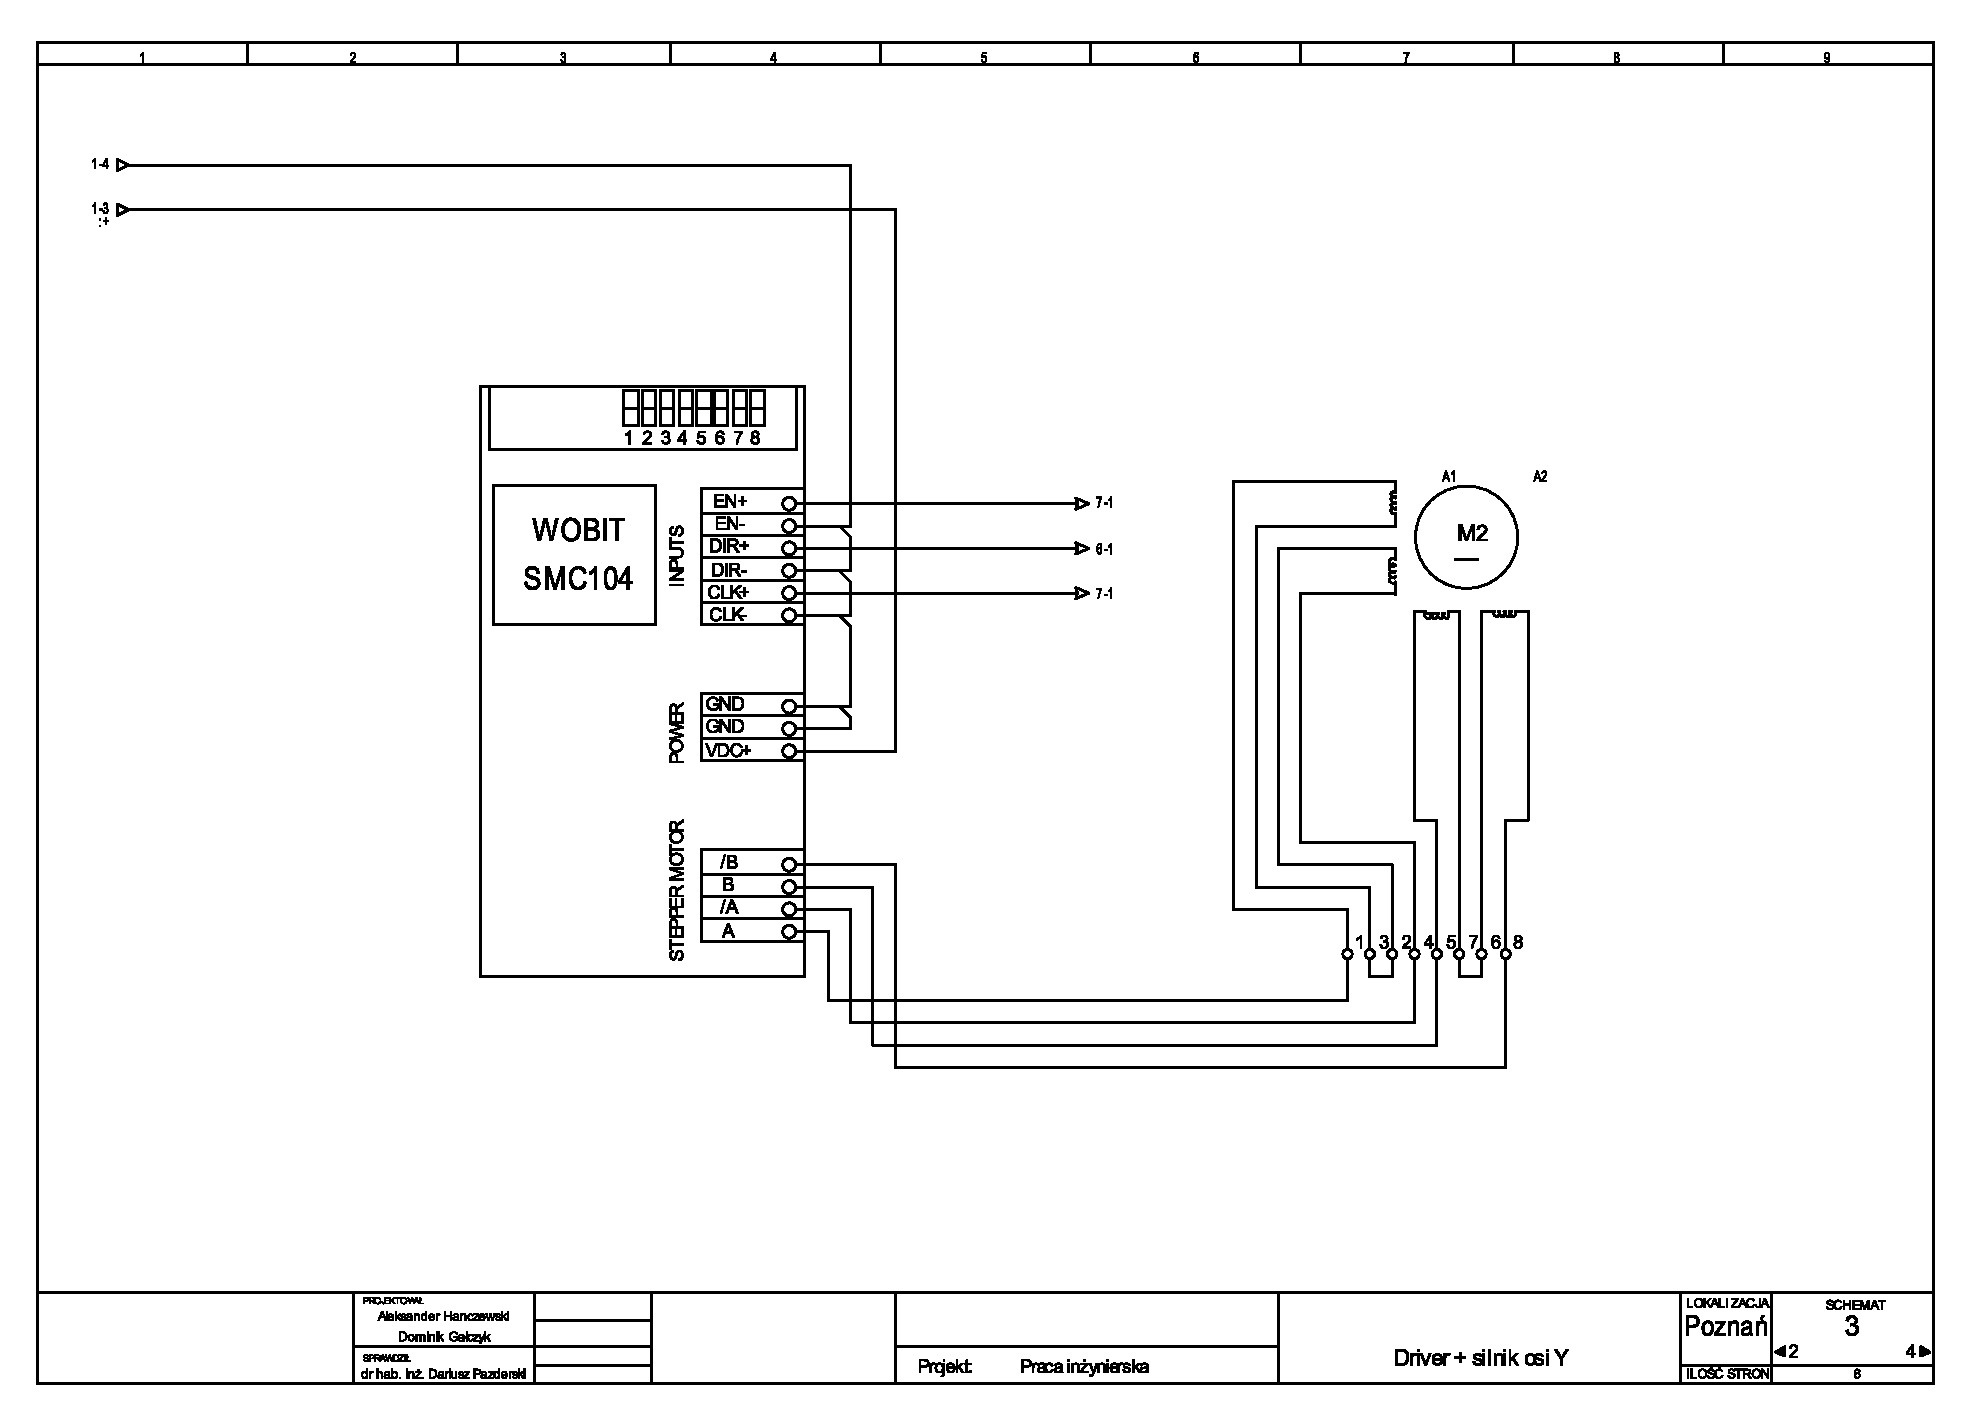
\includegraphics[width=0.85\textwidth]{pictures/schemat_elektryczny/Inżynierka (8).pdf}
\end{figure}

\begin{figure}[H]
    \centering
    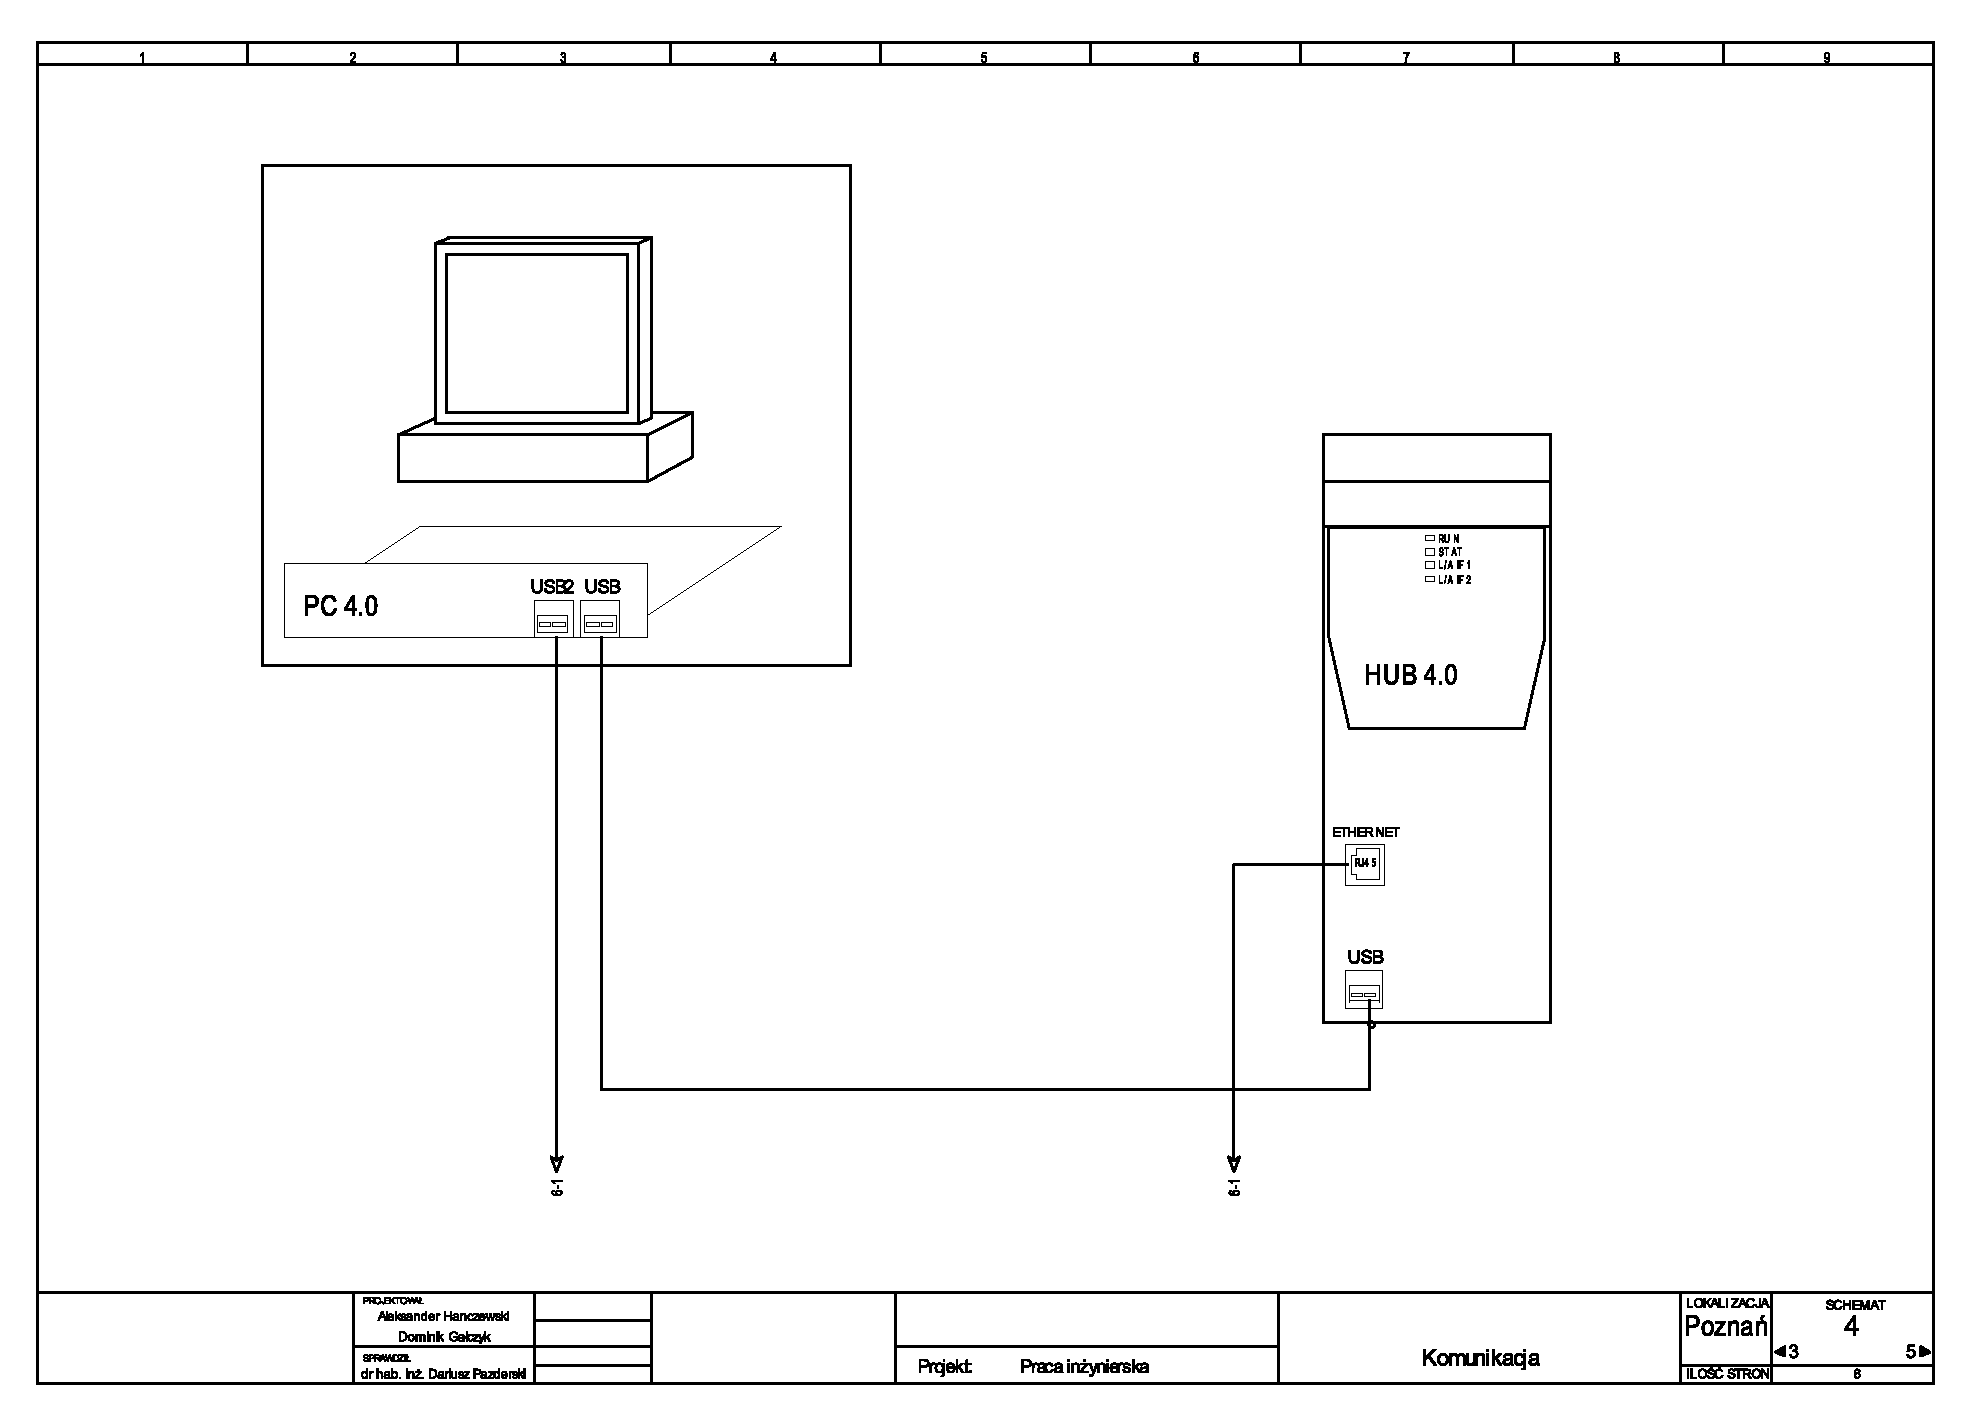
\includegraphics[width=0.85\textwidth]{pictures/schemat_elektryczny/Inżynierka (9).pdf}
\end{figure}

\begin{figure}[H]
    \centering
    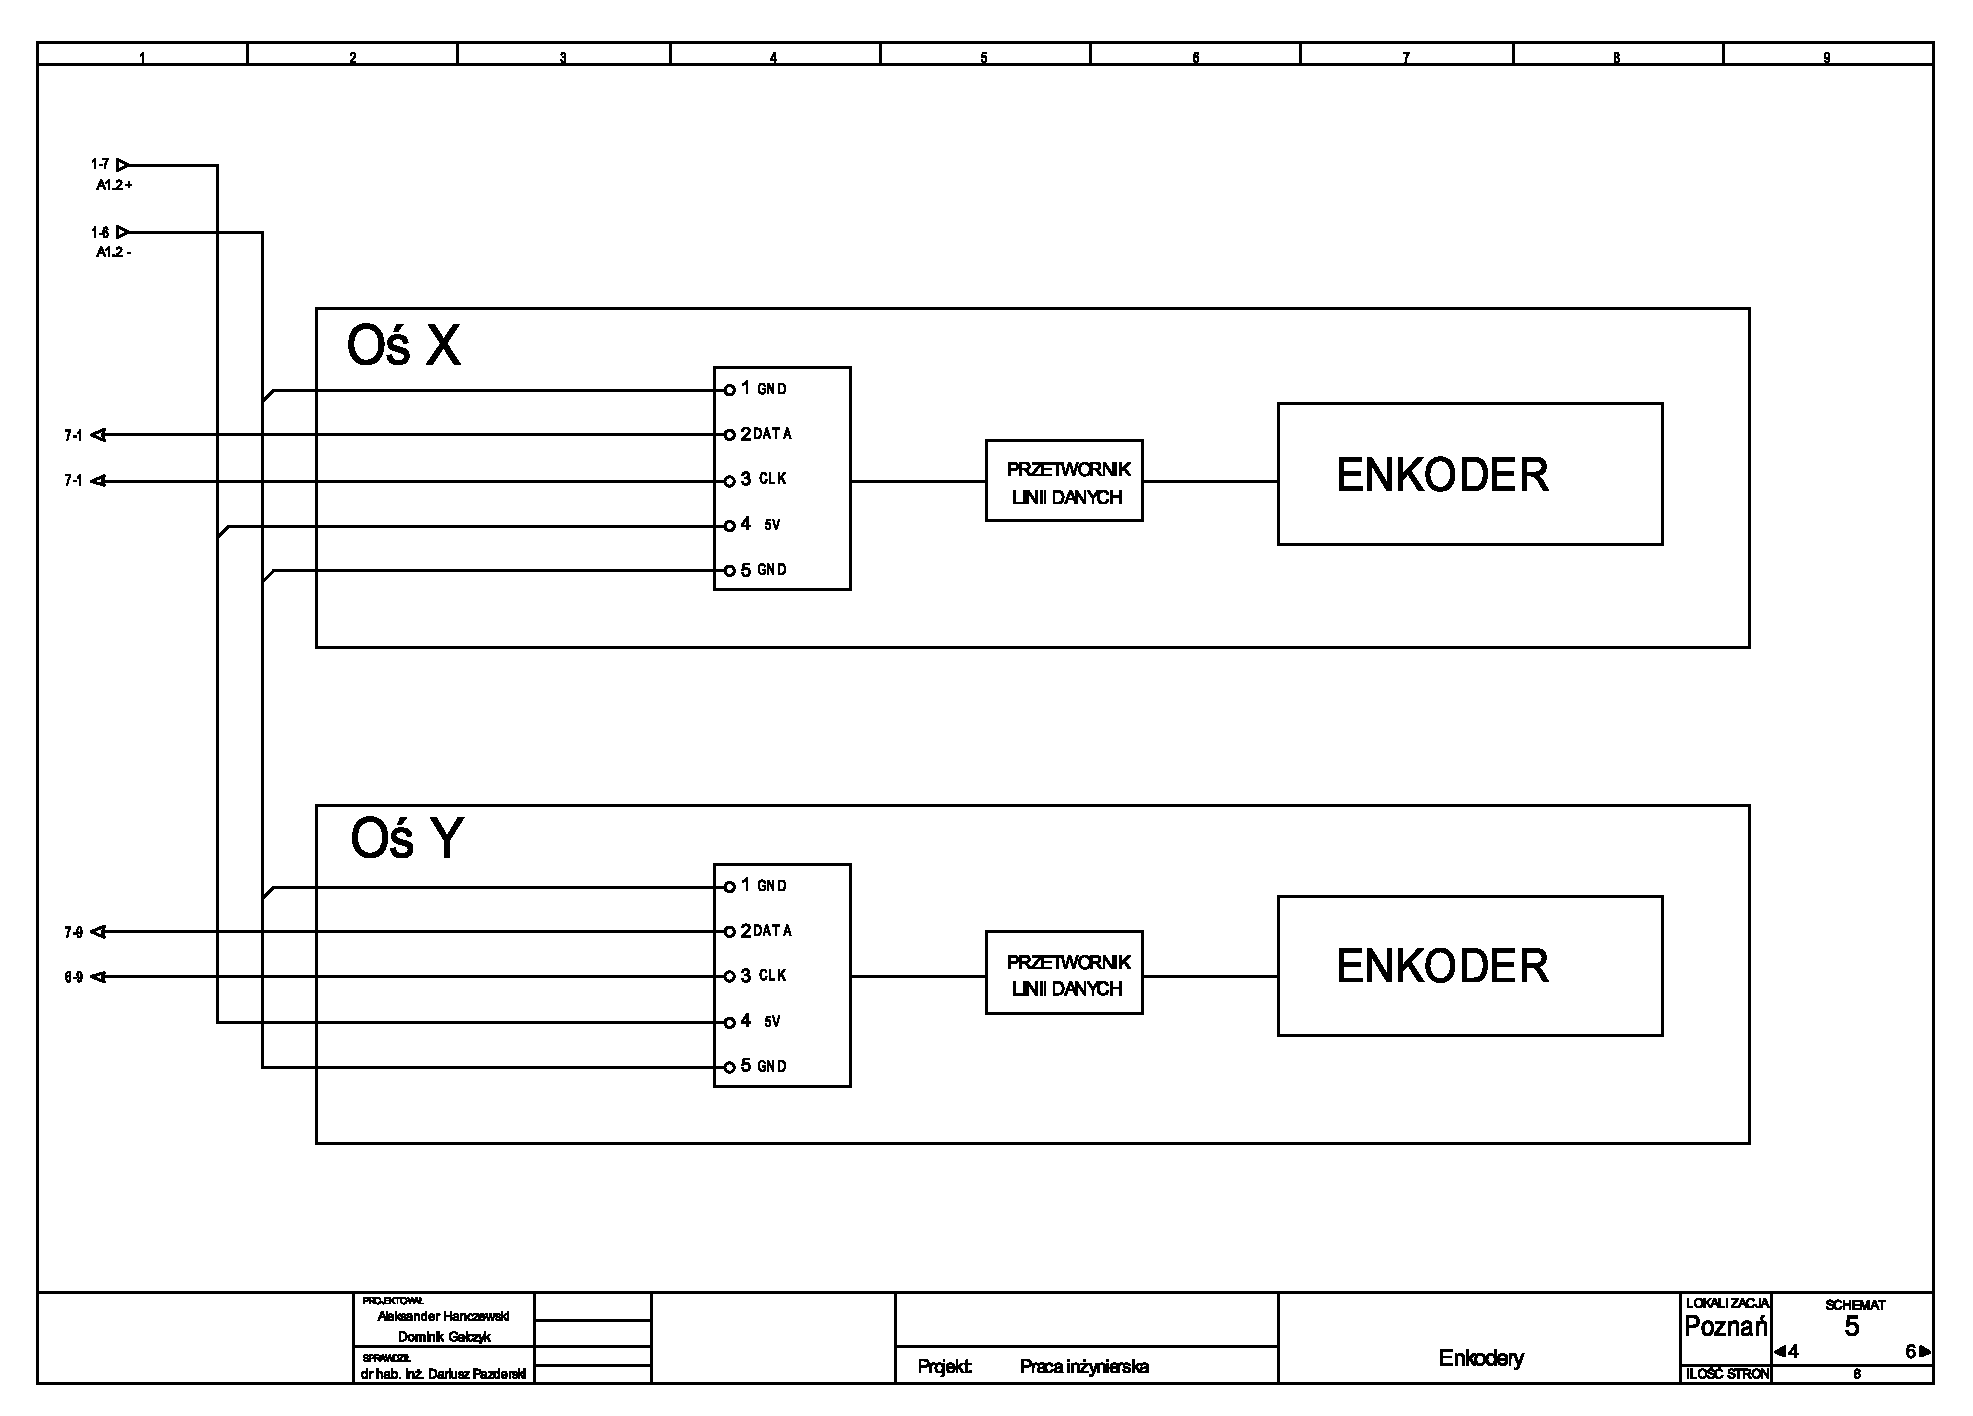
\includegraphics[width=0.85\textwidth]{pictures/schemat_elektryczny/Inżynierka (10).pdf}
\end{figure}

\begin{figure}[H]
    \centering
    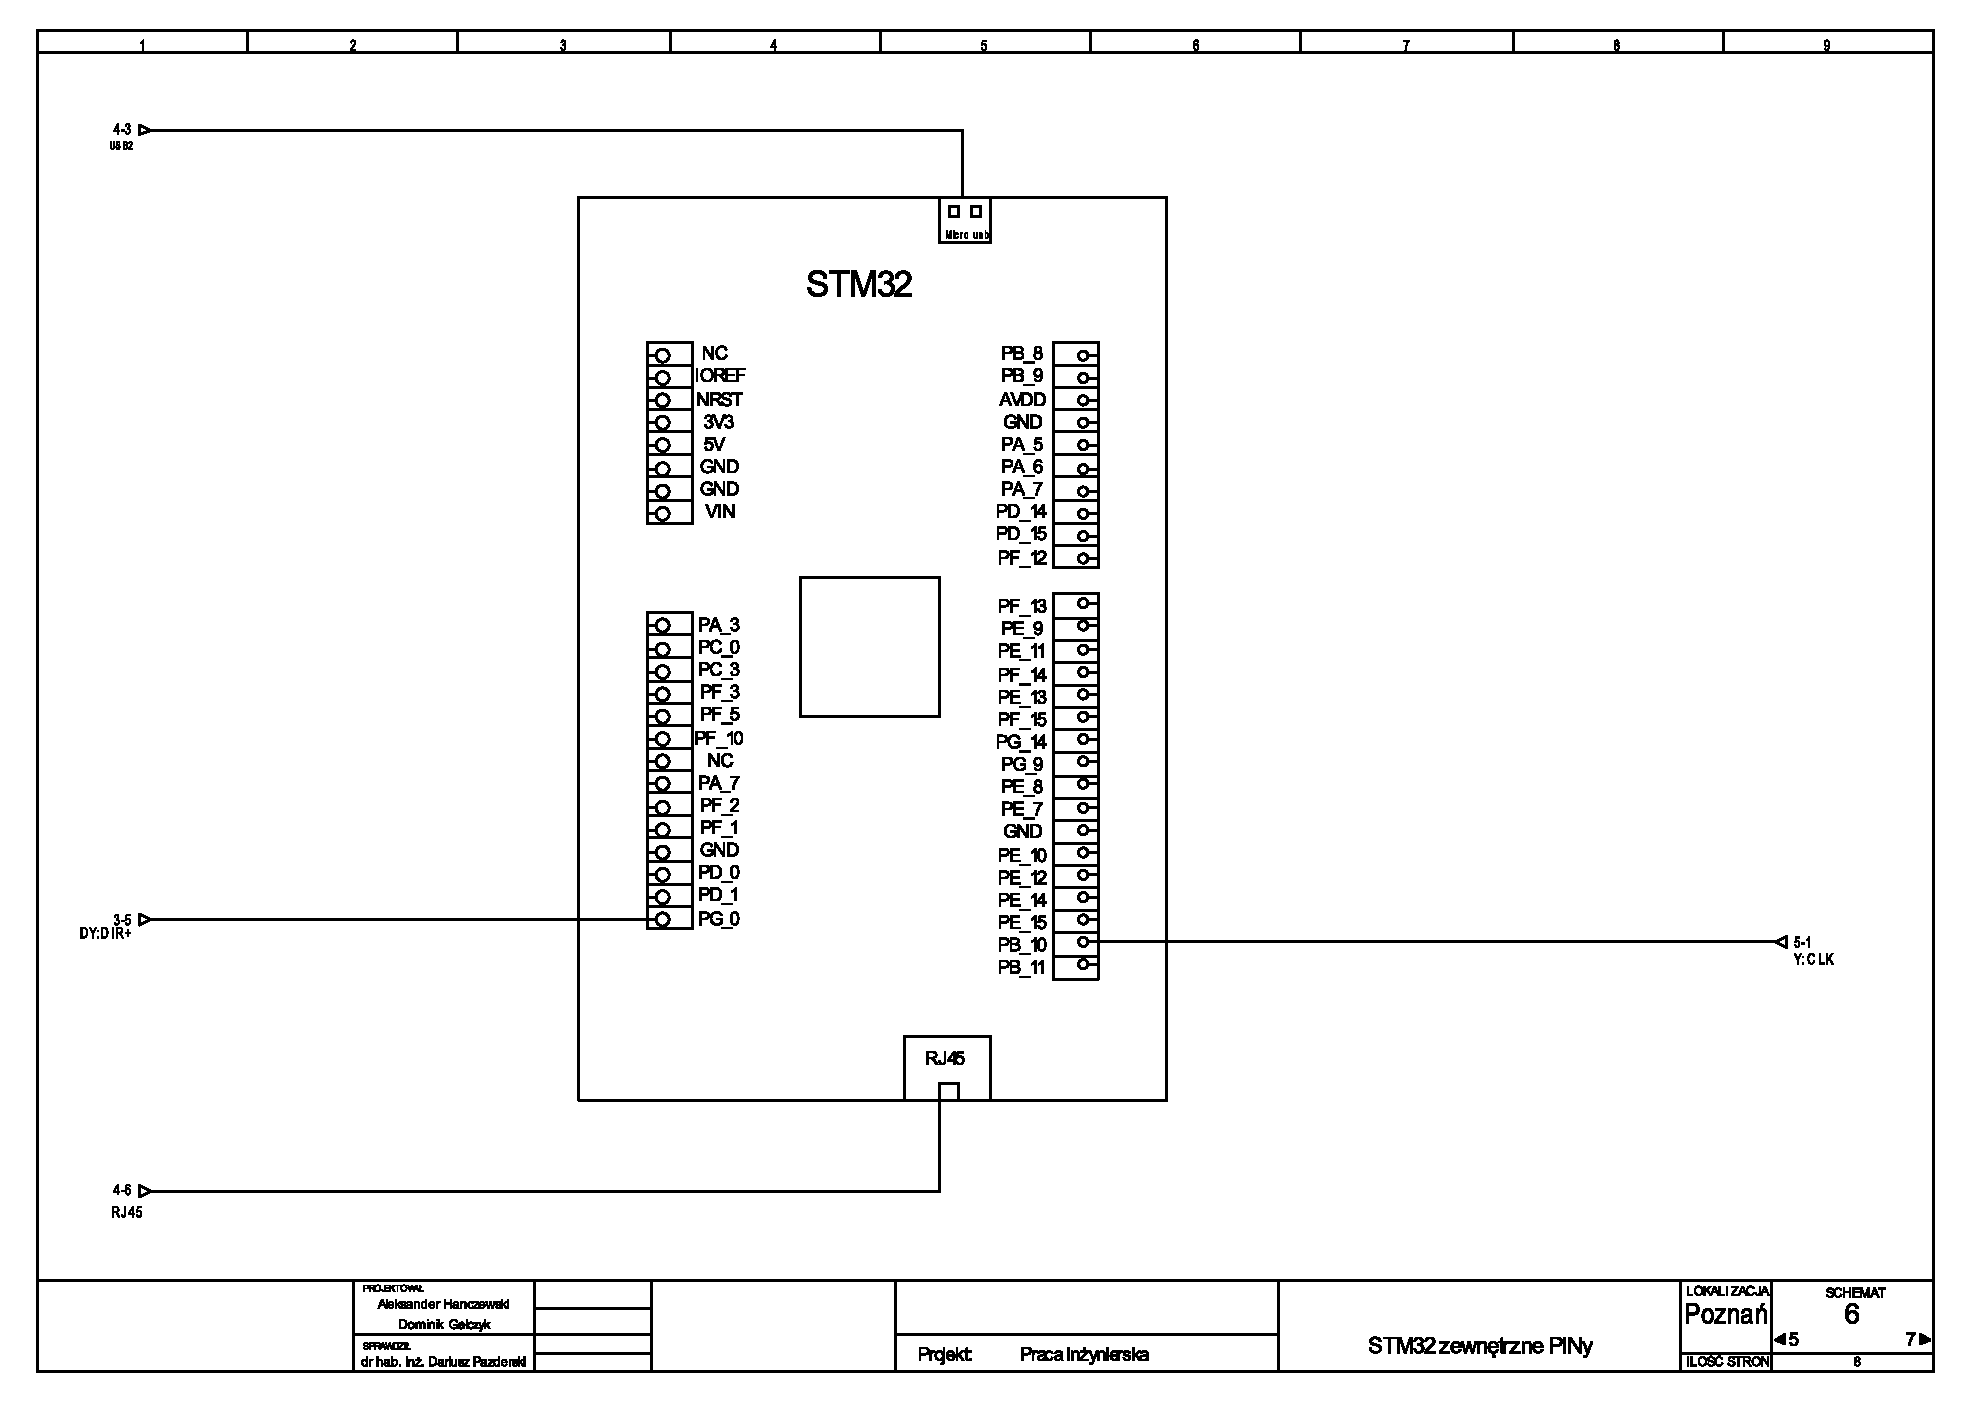
\includegraphics[width=0.85\textwidth]{pictures/schemat_elektryczny/Inżynierka (11).pdf}
\end{figure}

\begin{figure}[H]
    \centering
    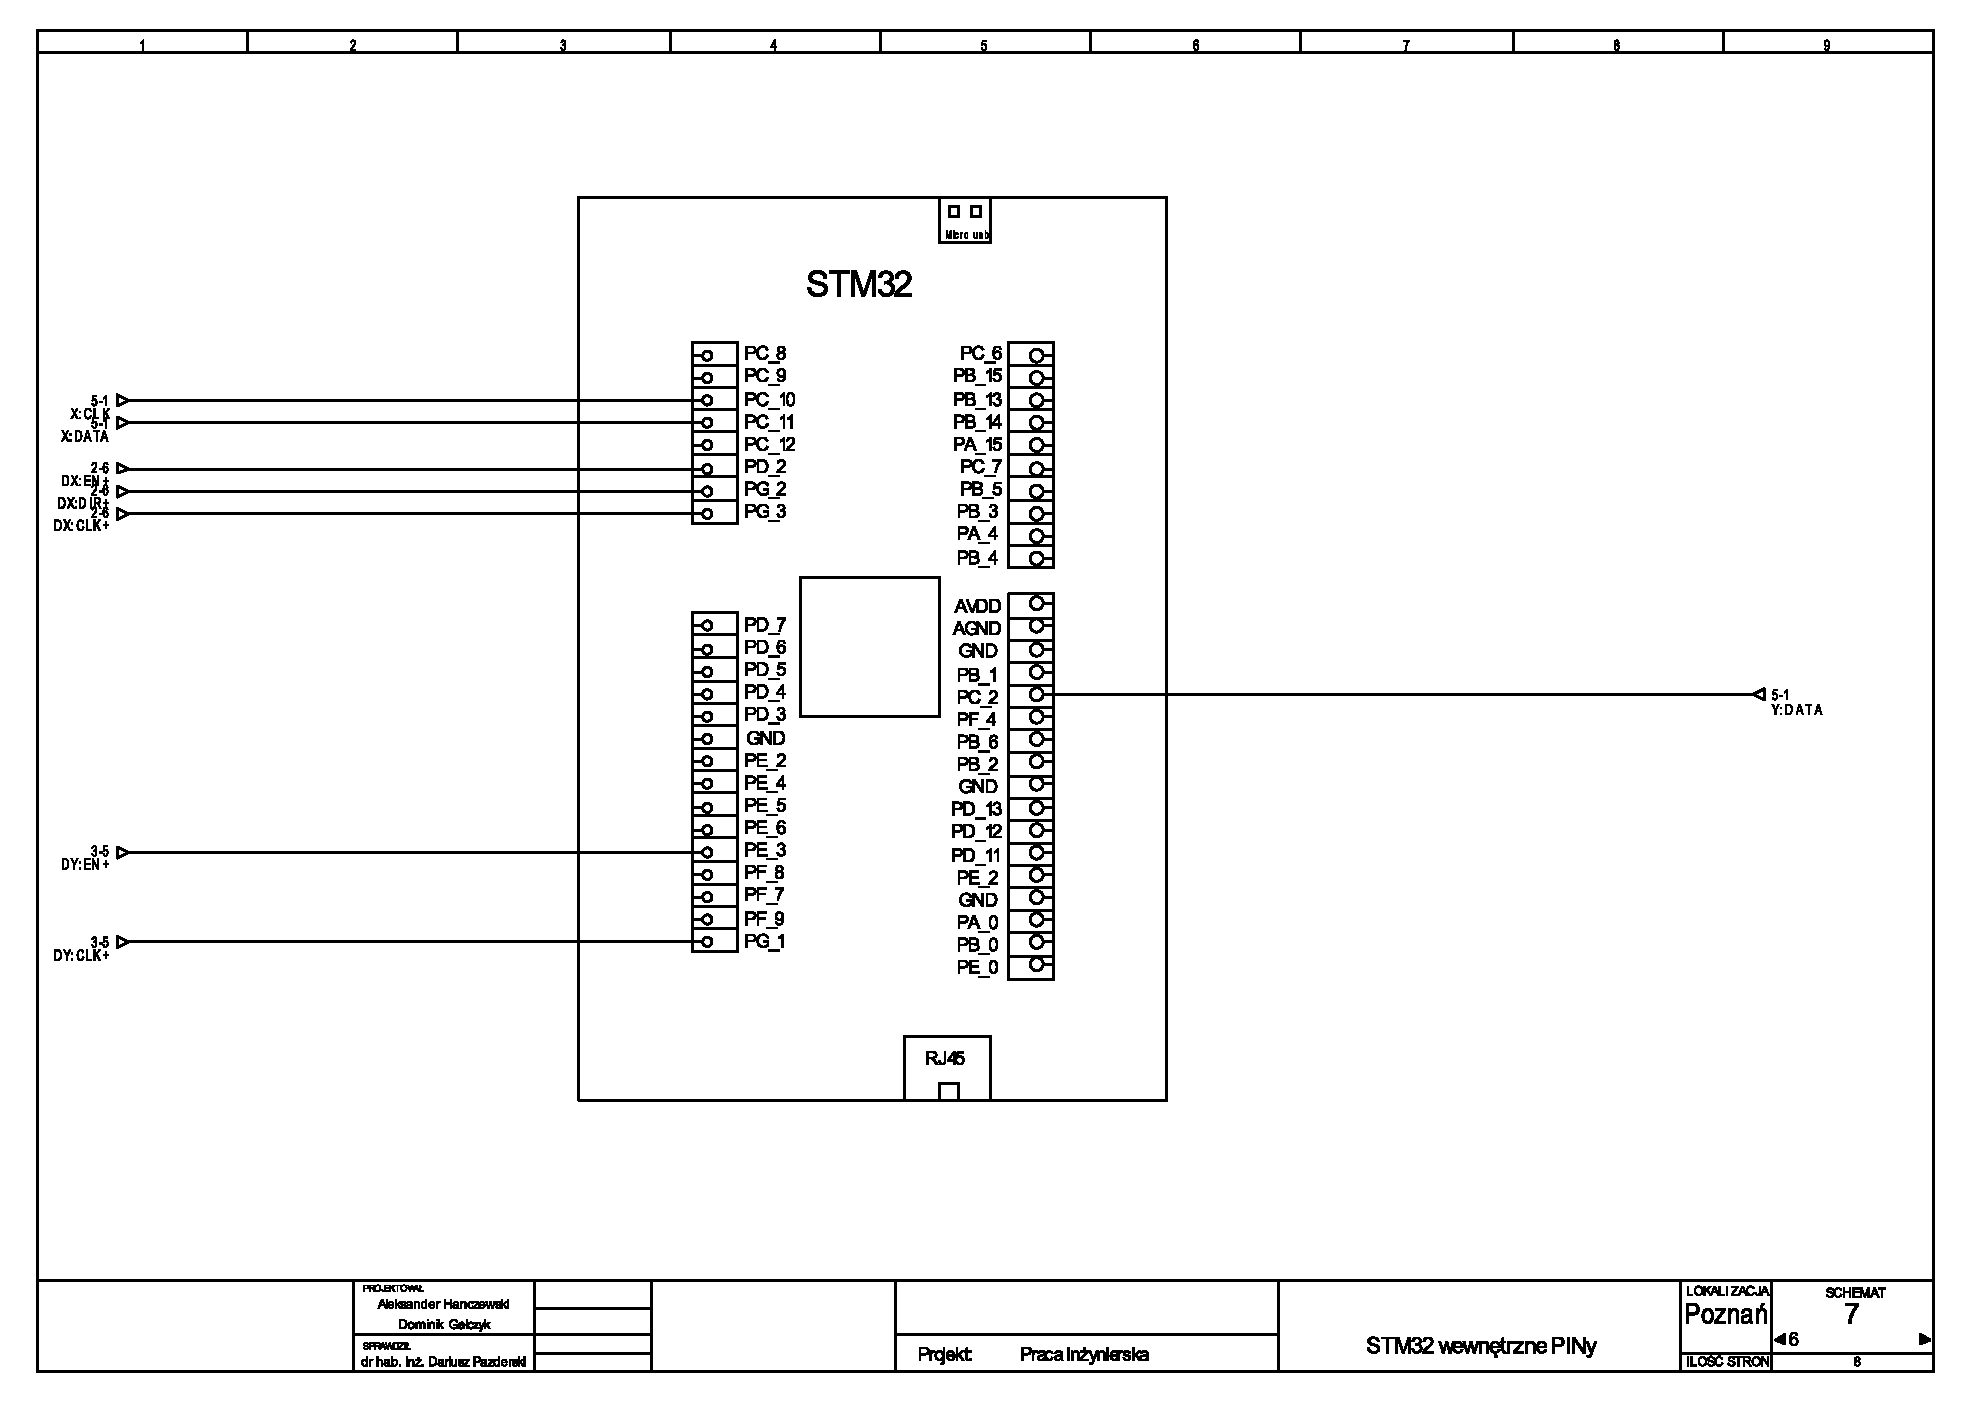
\includegraphics[width=0.85\textwidth]{pictures/schemat_elektryczny/Inżynierka (12).pdf}
\end{figure}

\chapter{Dodatek: Użyte kody w aplikacji}
Repozytorium online z aplikacją webową: \\ https://github.com/DGal02/AirInzynierkaReact2024 \\
Repozytorium online z aplikacją na STM32: \\ https://github.com/DGal02/AirInzynierkaSTM2024